% An exact diagram of the common uniform component in a finite block kernel.
% K(u,y) = epsilon/m + (1-epsilon)*R_u(y), epsilon=m*delta.
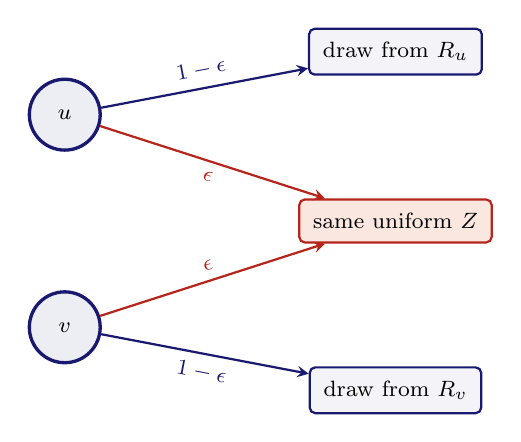
\begin{tikzpicture}[>=stealth,
 every node/.style={font=\footnotesize},
 state/.style={circle,draw=MidnightBlue,very thick,fill=MidnightBlue!8,minimum size=9mm},
 law/.style={rounded corners=2pt,draw=MidnightBlue,thick,fill=MidnightBlue!5,inner sep=5pt}]
\node[state] (u) at (0,1.35) {$u$};
\node[state] (v) at (0,-1.35) {$v$};
\node[law,fill=BrickRed!8,draw=BrickRed] (z) at (4.2,0) {same uniform $Z$};
\node[law] (ru) at (4.2,2.15) {draw from $R_u$};
\node[law] (rv) at (4.2,-2.15) {draw from $R_v$};
\draw[->,thick,BrickRed] (u) -- node[below,sloped] {$\epsilon$} (z);
\draw[->,thick,BrickRed] (v) -- node[above,sloped] {$\epsilon$} (z);
\draw[->,thick,MidnightBlue] (u) -- node[above,sloped] {$1-\epsilon$} (ru);
\draw[->,thick,MidnightBlue] (v) -- node[below,sloped] {$1-\epsilon$} (rv);
\end{tikzpicture}
